\chapter{Desarrollo Experimental}

\section{Experimento 1: Contrastación de Voltímetro Analógico}
Se montó un esquema en paralelo entre la fuente, el multímetro analógico UNIVO y el patrón digital Pro'sKit MT-1210. 

Se procedió a variar la tensión de la fuente, alineando la aguja del UNIVO exactamente sobre las divisiones de la escala ($V_L$), y tomando la lectura del patrón digital ($V_P$). Se efectuó una pasada ascendente y una descendente para contemplar histéresis y rozamiento mecánico del galvanómetro.

\begin{figure}[H]
    \centering
    \begin{subfigure}[b]{0.45\textwidth}
        \centering
        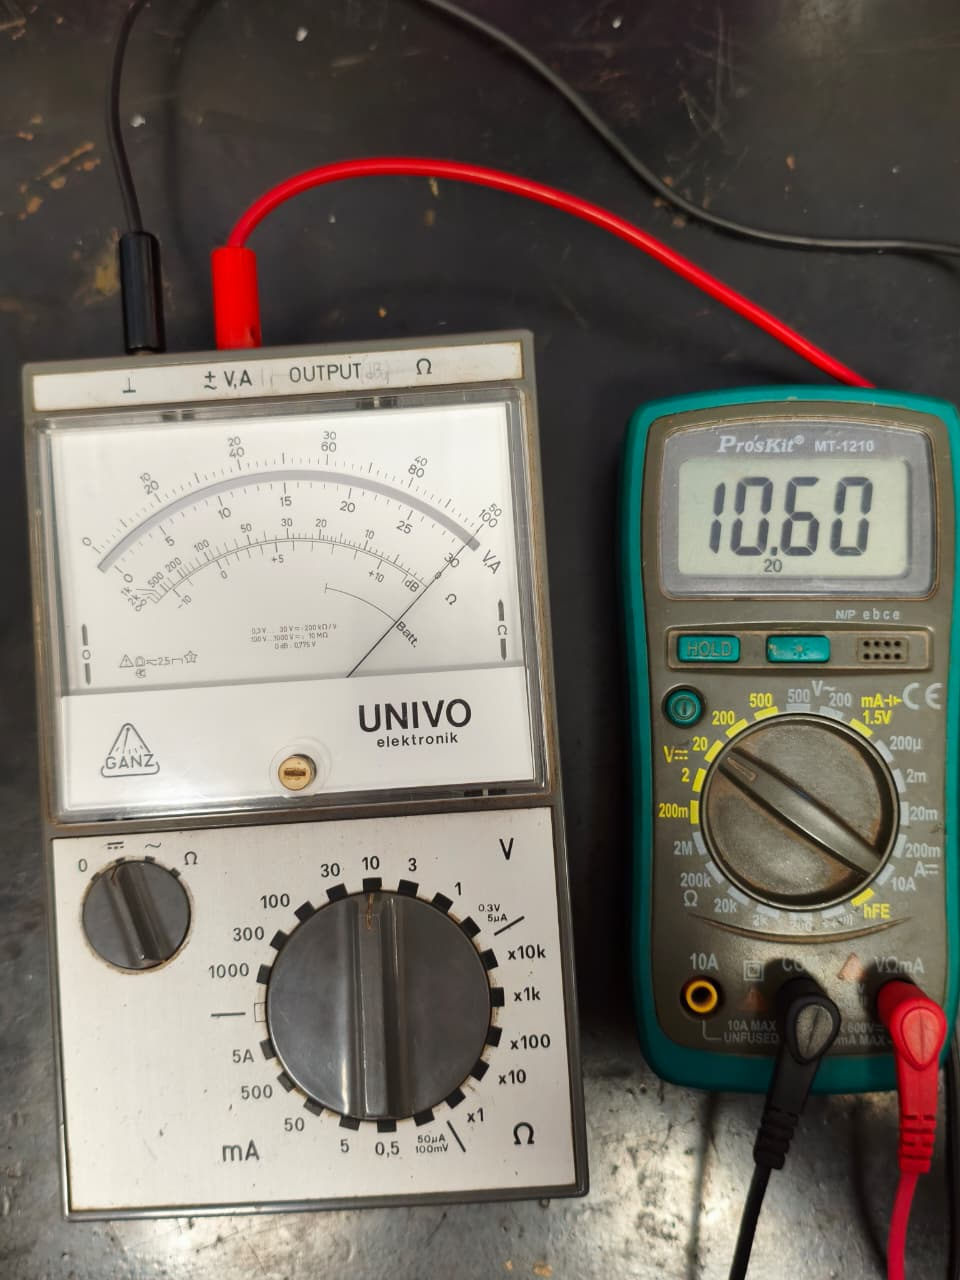
\includegraphics[width=\textwidth]{pictures/Constrastacion_voltimetro_analogico.jpeg}
        \caption{Montaje de contrastación en paralelo.}
    \end{subfigure}
    \hfill
    \begin{subfigure}[b]{0.45\textwidth}
        \centering
        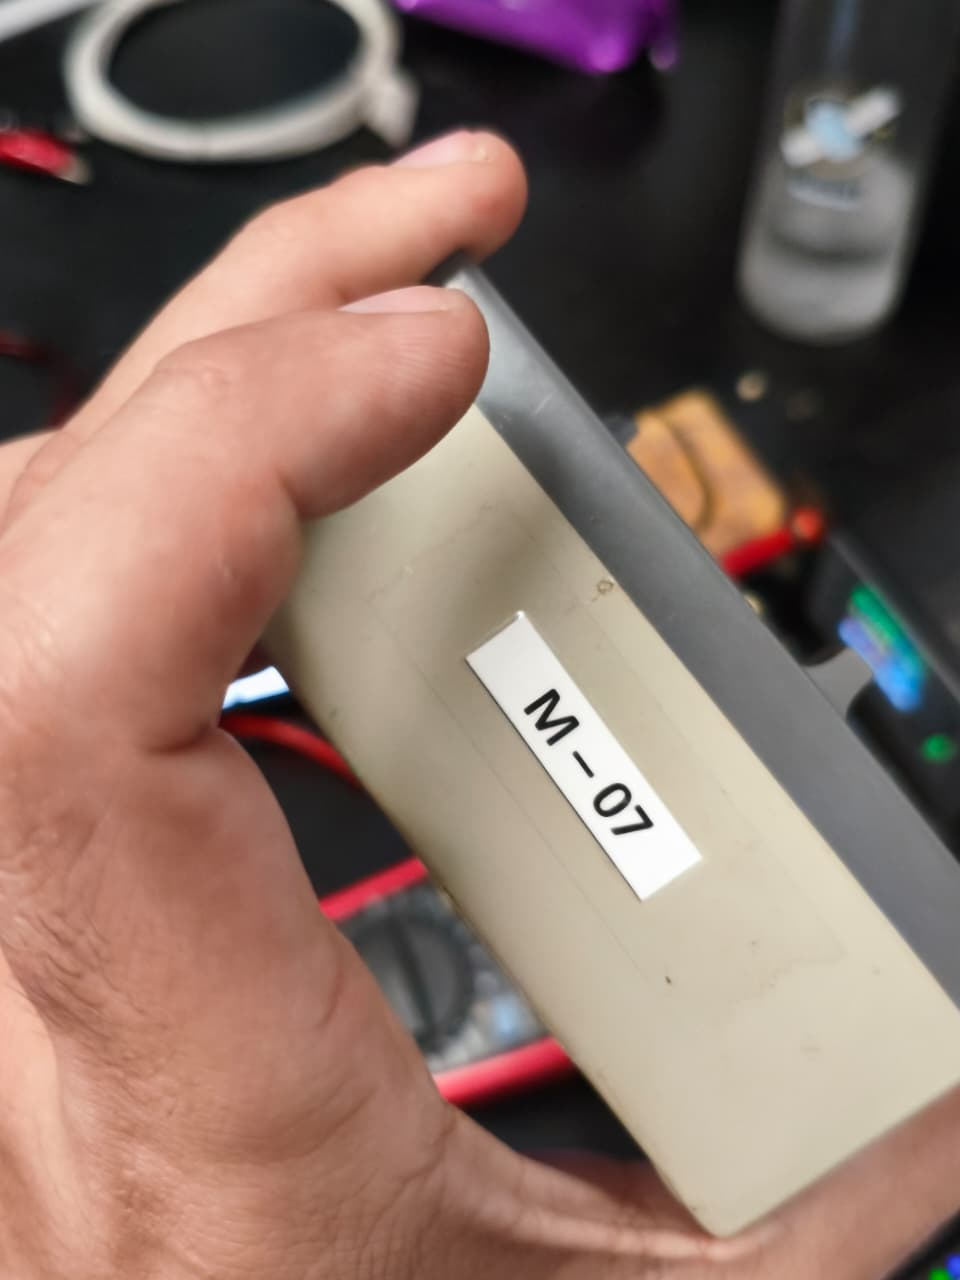
\includegraphics[width=\textwidth]{pictures/Comprobacion_serialnumber_volt_analogico.jpeg}
        \caption{Identificación del instrumento bajo prueba.}
    \end{subfigure}
    \caption{Proceso de contrastación del multímetro analógico UNIVO.}
\end{figure}

\begin{table}[H]
    \centering
    \resizebox{\textwidth}{!}{
    \begin{tabular}{|c|c|c|c|c|c|c|c|c|c|c|}
        \hline
        $V_L$ [$\V$] & 1 & 2 & 3 & 4 & 5 & 6 & 7 & 8 & 9 & 10 \\ \hline
        $V_P$ (hacia arriba) & 1,01 & 2,14 & 3,20 & 4,25 & 5,32 & 6,39 & 7,46 & 8,52 & 9,59 & 10,60 \\ \hline
        $V_P$ (hacia abajo) & 0,99 & 2,11 & 3,17 & 4,23 & 5,31 & 6,38 & 7,45 & 8,51 & 9,57 & 10,60 \\ \hline
        $\Delta V$ (mayor valor) & 0,01 & 0,14 & 0,20 & 0,25 & 0,32 & 0,39 & 0,46 & 0,52 & 0,59 & 0,60 \\ \hline
    \end{tabular}}
    \caption{Valores obtenidos de la contrastación. $V_L$: indicado, $V_P$: patrón, $\Delta V$: Error absoluto.}
\end{table}

\subsection{Curva de Contrastación}
\begin{figure}[H]
    \centering
    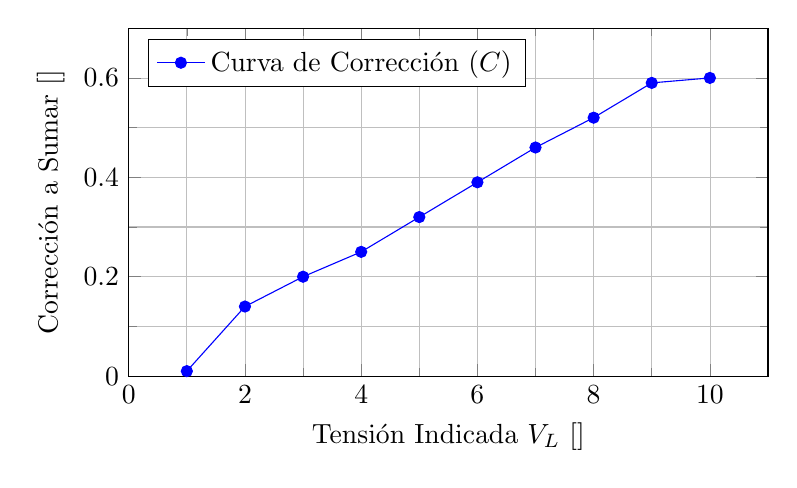
\begin{tikzpicture}
        \begin{axis}[
            width=0.8\textwidth,
            height=6cm,
            xlabel={Tensión Indicada $V_L$ [$\V$]},
            ylabel={Corrección a Sumar [$\V$]},
            xmin=0, xmax=11,
            ymin=0, ymax=0.7,
            grid=both,
            minor tick num=1,
            major grid style={line width=.2pt,draw=gray!50},
            legend pos=north west
        ]
        \addplot[color=blue, mark=*] coordinates {
            (1, 0.01)
            (2, 0.14)
            (3, 0.20)
            (4, 0.25)
            (5, 0.32)
            (6, 0.39)
            (7, 0.46)
            (8, 0.52)
            (9, 0.59)
            (10, 0.60)
        };
        \legend{Curva de Corrección ($C$)}
        \end{axis}
    \end{tikzpicture}
    \caption{Curva de contrastación: Valores a sumar al instrumento bajo prueba en función de su indicación.}
\end{figure}

\vspace{0.5cm}
\begin{figure}[H]
    \centering
    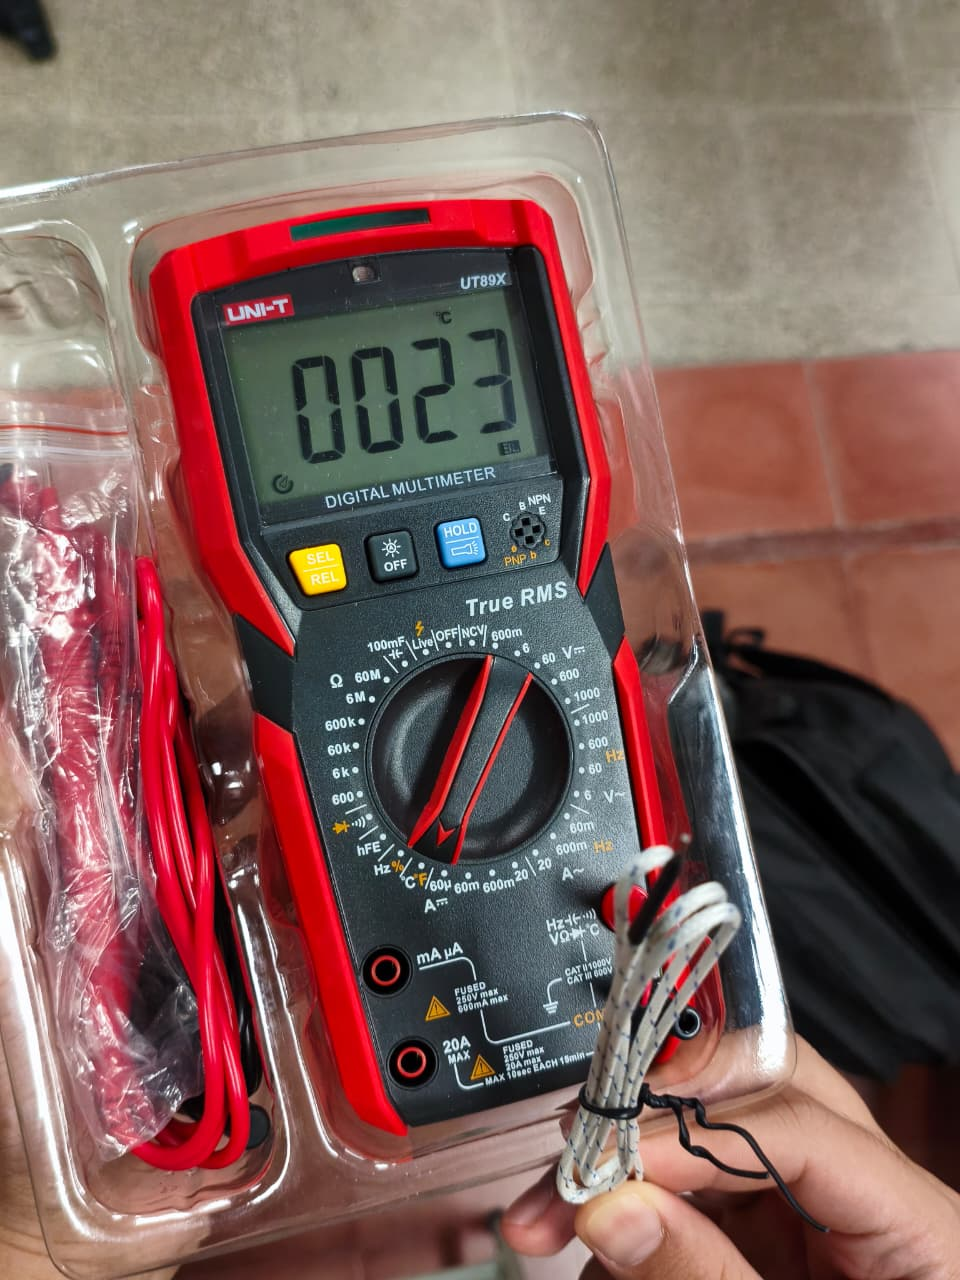
\includegraphics[width=0.4\textwidth]{pictures/Temperatura_ambiente.jpeg}
    \caption{Medición de la temperatura ambiente durante la experiencia.}
\end{figure}

\begin{table}[H]
    \centering
    \begin{tabular}{|p{4cm}|p{4cm}|c|c|}
        \hline
        \textbf{Inst. Contrastado} & \textbf{Patrón} & \textbf{Fecha y Hora} & \textbf{Operador} \\ \hline
        Marca: UNIVO \newline Nro: S/D & Marca: Pro'sKit \newline Nro: S/D & 09/04/2026 \newline 17:48 hs & Franco \newline Palombo \\ \hline
        \multicolumn{4}{|l|}{\textbf{Temperatura Ambiente:} 23 $\Celsius$} \\ \hline
    \end{tabular}
    \caption{Datos de trazabilidad de la contrastación.}
\end{table}

\subsection{Cálculo del Índice de Clase}
Del cuadro de datos, se identifica el Error Absoluto Máximo ($\Delta V = 0,60 \ \text{V}$ en $V_L = 10 \ \text{V}$) y se calcula el índice de clase:
\begin{equation}
    Clase = \frac{0,60}{10} \cdot 100 = 6 \percent
\end{equation}
\textit{(Redondear hacia arriba el resultado). Comprobación: El fabricante del UNIVO declara una Clase de $2,5$. ¿Guarda coherencia el valor obtenido?} \textbf{El valor obtenido no guarda coherencia con lo declarado por el fabricante. El instrumento presenta un índice de clase experimental del $6\%$, lo que significa que se encuentra fuera de especificación y requeriría una recalibración o reparación, ya que su error supera ampliamente el límite de $2,5\%$ del fondo de escala establecido para su correcto funcionamiento.}

\section{Experimento 2: Medición de Resistencia por 4 Terminales}
Se ajustó el generador de corriente (fuente SK150) para entregar una corriente de prueba constante. La probeta consiste en un arrollamiento no inductivo de cable (longitud $12\text{m} \pm 12\text{cm}$).

\begin{table}[H]
    \centering
    \begin{tabular}{|c|c|c|}
        \hline
        $V$ [$\mV$] & $I$ [$\mA$] & $R = V/I$ [$\ohm$] \\ \hline
        56,8 & 100,0 & 0,568 \\ \hline
    \end{tabular}
    \caption{Medición directa de tensión y corriente en la probeta.}
\end{table}

\begin{figure}[H]
    \centering
    \begin{subfigure}[b]{0.45\textwidth}
        \centering
        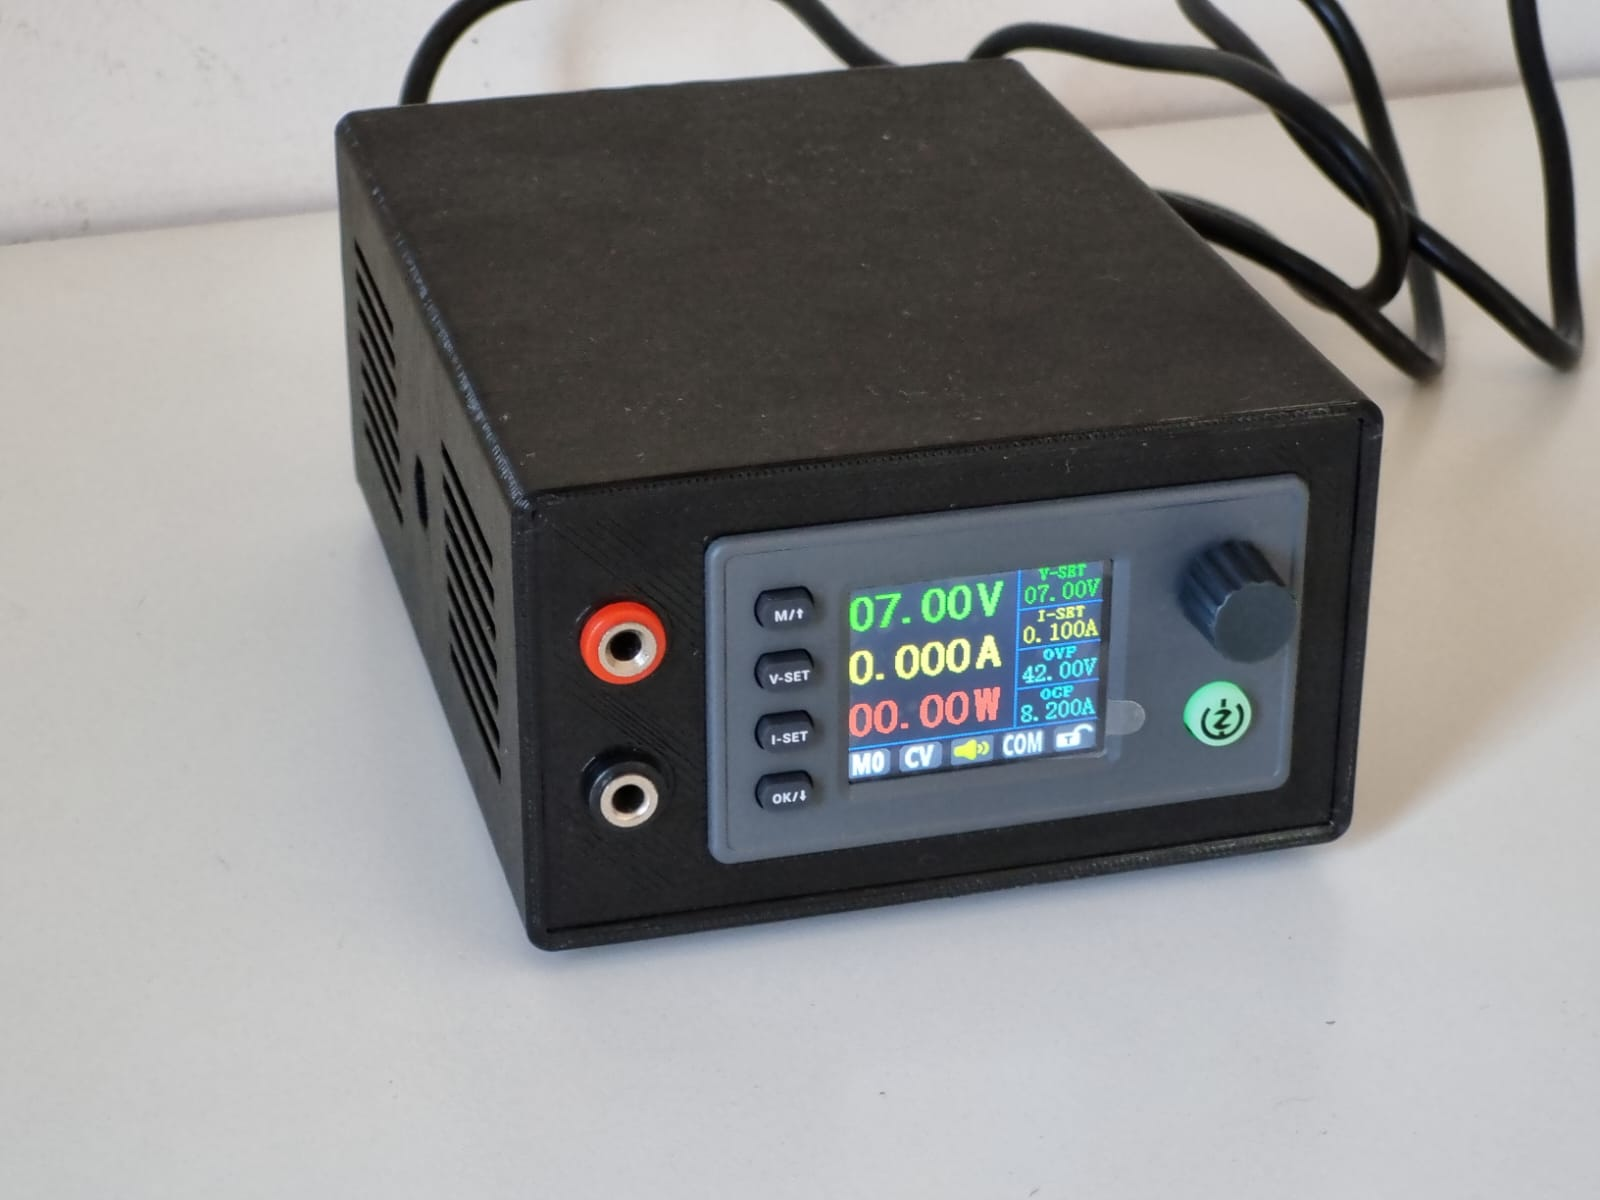
\includegraphics[width=\textwidth]{pictures/Fuente_sk150.jpeg}
        \caption{Fuente de corriente constante SK150.}
    \end{subfigure}
    \hfill
    \begin{subfigure}[b]{0.45\textwidth}
        \centering
        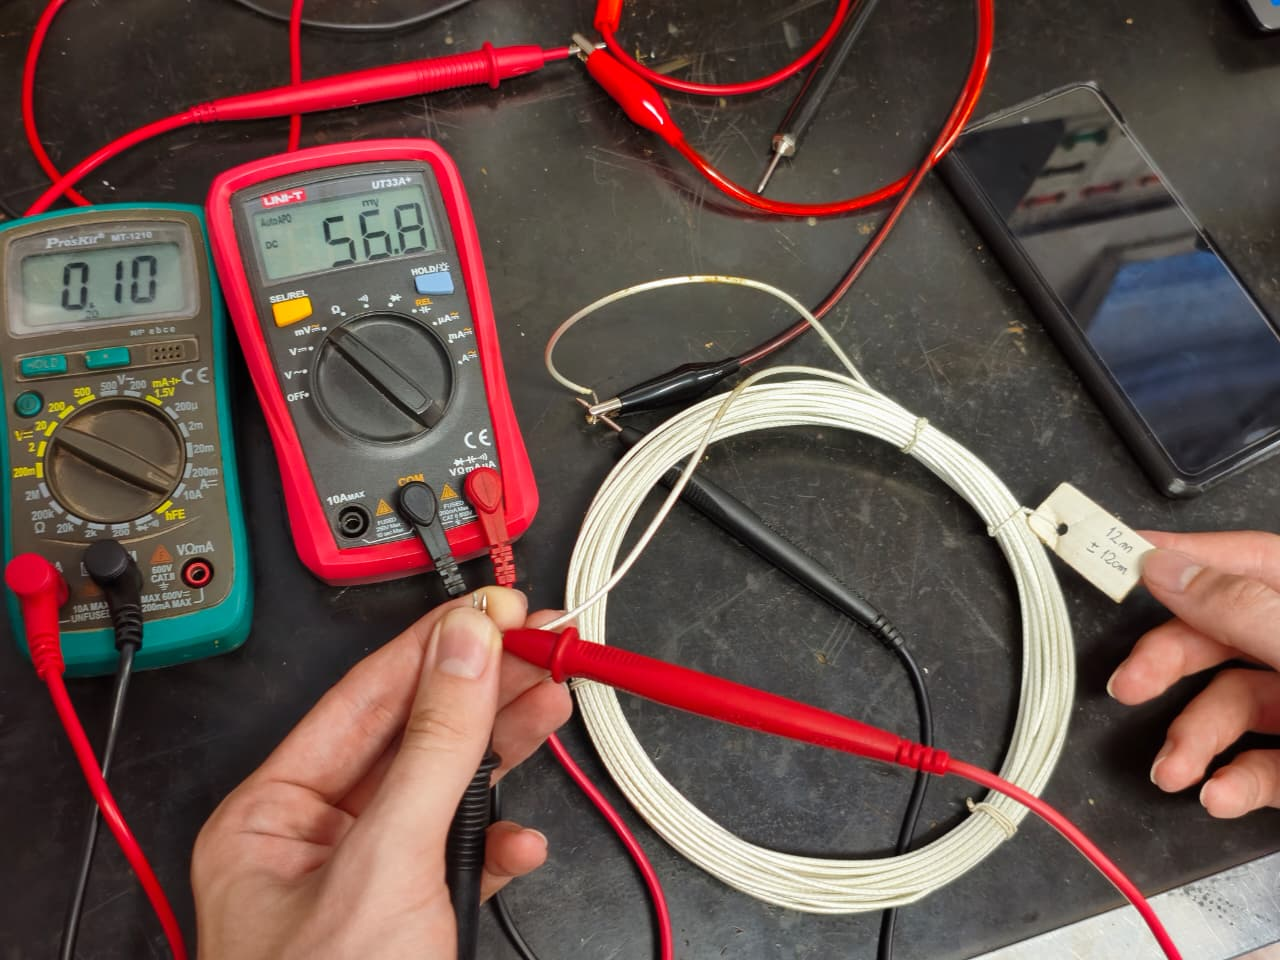
\includegraphics[width=\textwidth]{pictures/Medicion_Resistencia_4term.jpeg}
        \caption{Conexión de las 4 puntas sobre la probeta.}
    \end{subfigure}
    \caption{Montaje del experimento de 4 terminales, inyectando $100\mA$ y midiendo la caída de tensión en milivoltios.}
\end{figure}

\subsection{Cálculo de la Incertidumbre}
Los errores relativos parciales se suman para obtener el error relativo máximo total de la medición indirecta de $R$:
\begin{equation}
    \frac{\Delta R}{R} = \frac{\Delta V}{V} + \frac{\Delta I}{I}
\end{equation}

Las incertidumbres $\Delta V$ y $\Delta I$ se obtienen de los manuales de los instrumentos. Para el multímetro UNI-T UT33A+ (usado como milivoltímetro en rango $200\mV$), asumimos una exactitud típica de $\pm(0.5\% + 2 \text{ dig.})$. Para el Pro'sKit MT-1210 (usado como miliamperímetro en rango $200\mA$), asumimos $\pm(1.2\% + 2 \text{ dig.})$.

\begin{table}[H]
    \centering
    \resizebox{\textwidth}{!}{
    \begin{tabular}{|c|c|c|c|c|}
        \hline
        Magnitud & Valor Medido & Incertidumbre Abs. ($\Delta x$) & Inc. Relativa $\left(\frac{\Delta x}{X}\right)$ & Inc. Rel. Porcentual $\left(\frac{\Delta x}{X} \cdot 100\right)$ \\ \hline
        $V$ & $56,8 \mV$ & $0,484 \mV$ & $0,0085$ & $0,85\%$ \\ \hline
        $I$ & $100,0 \mA$ & $1,4 \mA$ & $0,0140$ & $1,40\%$ \\ \hline
        $R = V/I$ & $0,568 \ohm$ & $0,013 \ohm$ & $0,0225$ & $2,25\%$ \\ \hline
    \end{tabular}}
    \caption{Desglose de valores de incertidumbre.}
\end{table}

\textbf{Resultado Final:} $R = (0,568 \pm 0,013) \ \ohm$

\section{Experimento 3: Resistencia de un Sistema de Puesta a Tierra}
\textbf{Fecha de la experiencia:} Jueves 27 de Marzo en el horario de clases.

Para medir la resistencia de la jabalina del "Laboratorio Central de Electrónica" (caja ubicada debajo del pizarrón), se empleó el telurímetro UNI-T UT522 con un montaje de electrodos auxiliares sobre paños húmedos en el piso del pasillo exterior, emulando una malla conductora. Se seleccionó inicialmente el rango de $4000\ohm$.

\begin{itemize}
    \item \textbf{Valor leído $R(Jabalina)$:} \dots $\ohm$
\end{itemize}

De acuerdo al manual del instrumento, las especificaciones son:
\begin{itemize}
    \item Rango $40\ohm$: $\pm(2.0\% + 20)$
    \item Rangos $400\ohm$ y $4000\ohm$: $\pm(2.0\% + 3)$
\end{itemize}

Considerando la lectura obtenida, la incertidumbre presente en la medición es:
\begin{itemize}
    \item \textbf{$R_j$ (con incertidumbre):} $\dots \pm \dots \ \ohm$
\end{itemize}
